\begin{figure}[htb]
	\centering
	\subfigure[Original frame]{
	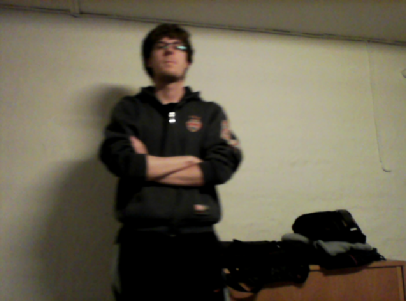
\includegraphics[scale=0.65]{grayscale/grayscale_1}
	\label{fig:grayscale_1}}
	\quad
	\subfigure[After subtraction]{
	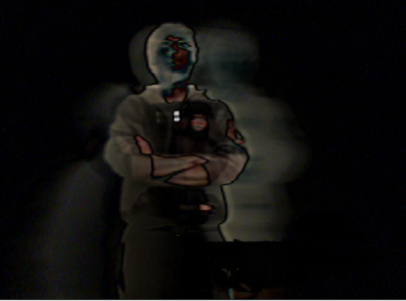
\includegraphics[scale=0.65]{grayscale/grayscale_2}
	\label{fig:grayscale_2}}
	\subfigure[After grayscale filter is applied]{
	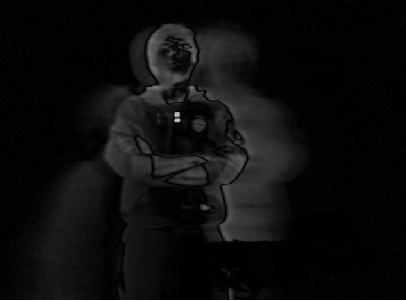
\includegraphics[scale=0.65]{grayscale/grayscale_3}
	\label{fig:grayscale_3}}
	\quad
	\subfigure[After threshold is applied]{
	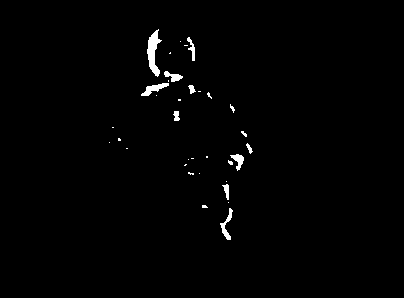
\includegraphics[scale=0.65]{threshold/threshold_1}
	\label{fig:threshold_1}}
	\subfigure[After dilation and erosion]{
	
\includegraphics[scale=0.65]{dilate_erode/dilate_erode_1}
	\label{fig:dilate_erode_1}}
	\quad
	\subfigure[After bounding box is drawn]{
	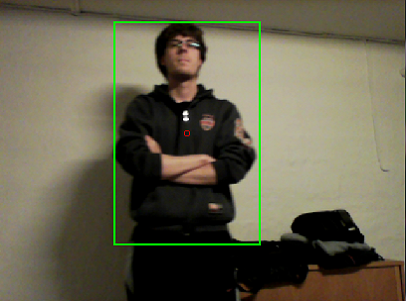
\includegraphics[scale=0.65]{bounding_box/bounding_box_1}
	\label{fig:bounding_box_1}}
	\caption{Object detection example}
	\label{fig:object_detection_example}
\end{figure}

\begin{figure}[htb]
	\centering
	\subfigure[Time (in seconds) needed to multiply two $300 \times 300$ size matrices in Java and Python on a laptop]{
	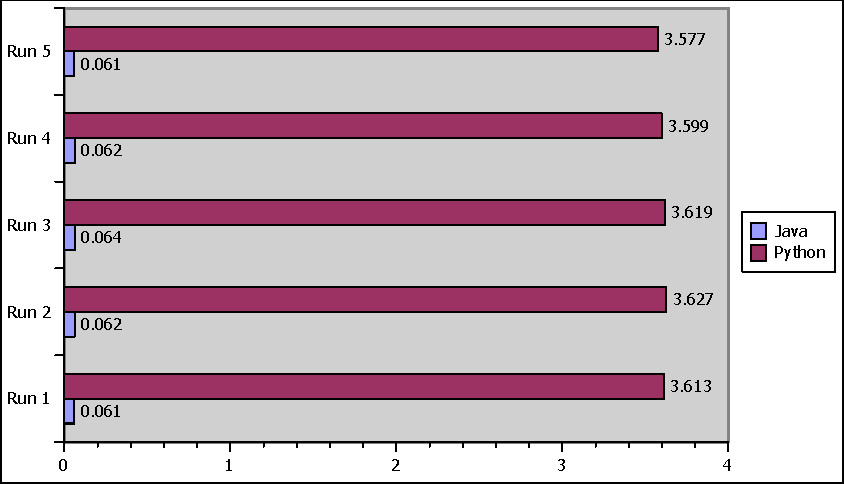
\includegraphics[scale=0.95]{benchmark/benchmark_1}
	\label{fig:benchmark_1}}
	\quad
	\subfigure[Time (in seconds) needed to multiply two $300 \times 300$ size matrices in Java and Python on a Raspberry Pi computer]{
	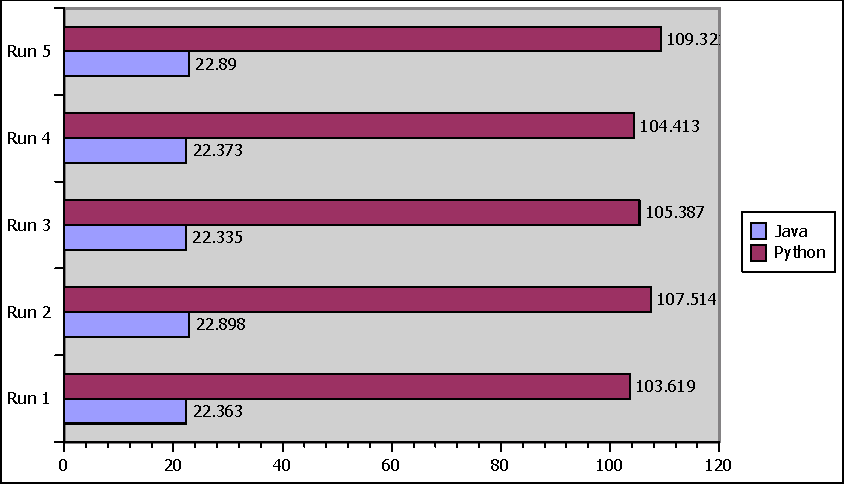
\includegraphics[scale=0.95]{benchmark/benchmark_2}
	\label{fig:benchmark_2}}
	\caption{Benchmark of matrix multiplication of two $300 \times 300$ size matrices}
	\label{fig:benchmark_multiplication}
\end{figure}

\begin{figure}[htb]
	\centering
	\subfigure[Average time (in seconds) needed to process images in Java and Python on a laptop]{
	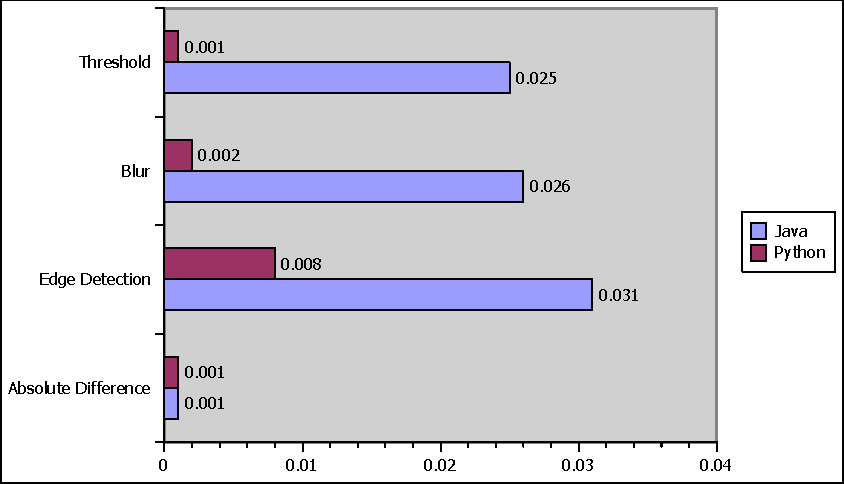
\includegraphics[scale=0.95]{benchmark/benchmark_3}
	\label{fig:benchmark_3}}
	\quad
	\subfigure[Average time (in seconds) needed to process images in Java and Python on a Raspberry Pi computer]{
	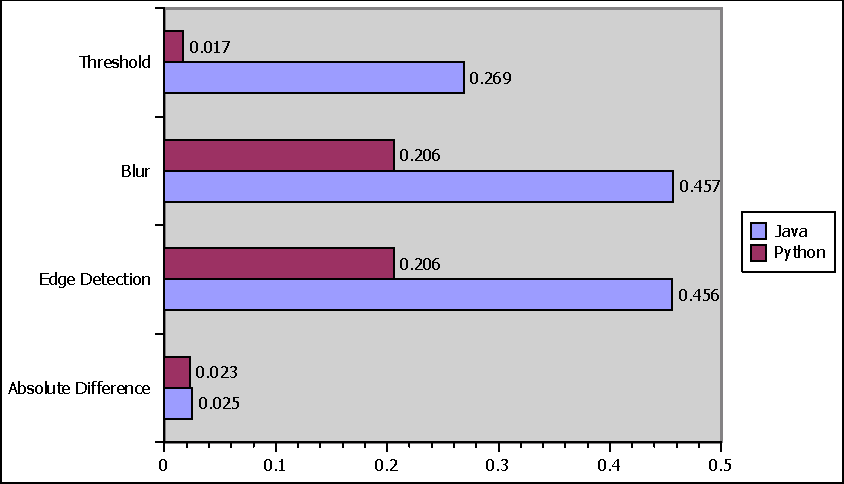
\includegraphics[scale=0.95]{benchmark/benchmark_4}
	\label{fig:benchmark_4}}
	\caption{Benchmark of image processing}
	\label{fig:benchmark_image_processing}
\end{figure}